\documentclass{standalone}
\usepackage{pgfplots}
\pgfplotsset{compat=1.15}
% Grouping the common style settings here to make the code below easier to read
\pgfkeys{/pgfplots/Axis Style/.style={
    width=13.5cm, height=5cm,
    axis x line=center, 
    axis y line=middle, 
    samples=100,
    ymin=-1.5, ymax=1.5,
    xmin=-3.2, xmax=3.2,
    domain=-pi:pi
}}

\begin{document}
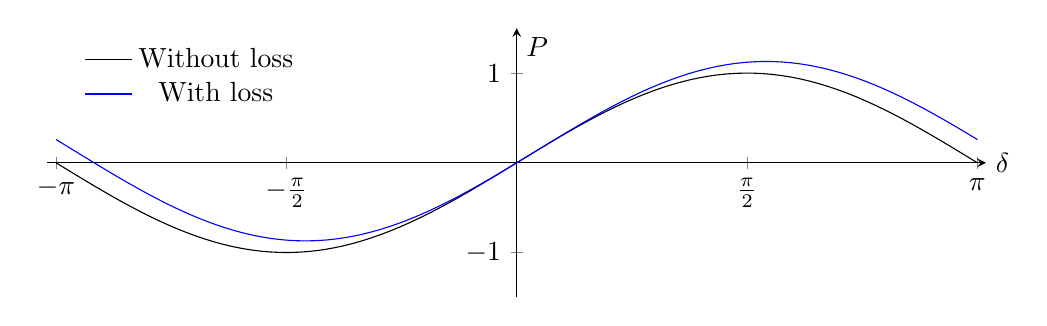
\begin{tikzpicture}
\begin{axis}[legend style={draw=none},
    Axis Style,
    xtick={
        -3.14159, -1.5708,
        1.5708, 3.14159
    },
    xticklabels={
        $-\pi$, $-\frac{\pi}{2}$,
        $\frac{\pi}{2}$, $\pi$
    },
    every axis x label/.style={at={(current axis.right of origin)},anchor=west},
    xlabel={$\delta$},
    ylabel={$P$},
    legend pos=north west
 ]
\addplot [mark=none, thin, black] {sin(deg(x))}
        %node[pos=.83, below] {Real power flow}
        ;
\addplot [mark=none, thin, blue] {sin(deg(x-0.13)) + sin(deg(0.13)}
         %node[pos=.63, above] {Real power flow}
         ;
\legend{Without loss, With loss}

\end{axis}
\end{tikzpicture}


\end{document}